\chapter{What is the LMD Martian Mesoscale Model?}\label{whatis}

\vk
This chapter comprises slightly edited excerpts from \textit{Spiga and Forget} [2009]\nocite{Spig:09}, dedicated to a general scientific and technical description of the LMD Martian Mesoscale Model, of its design and capabilities. Further details can be found in the reference \textit{Spiga and Forget} [2009]\nocite{Spig:09} paper and subsequent papers about mesoscale applications: e.g., \textit{Spiga and Lewis} [2010]\nocite{Spig:10dust} and \textit{Spiga et al.} [2011]\nocite{Spig:11ti}. Figure~\ref{modelstructure} summarizes the main points detailed in this introduction. This chapter is intended both for beginners and advanced users of the LMD Martian Mesoscale Model.

\begin{center}
\begin{figure}[p] 
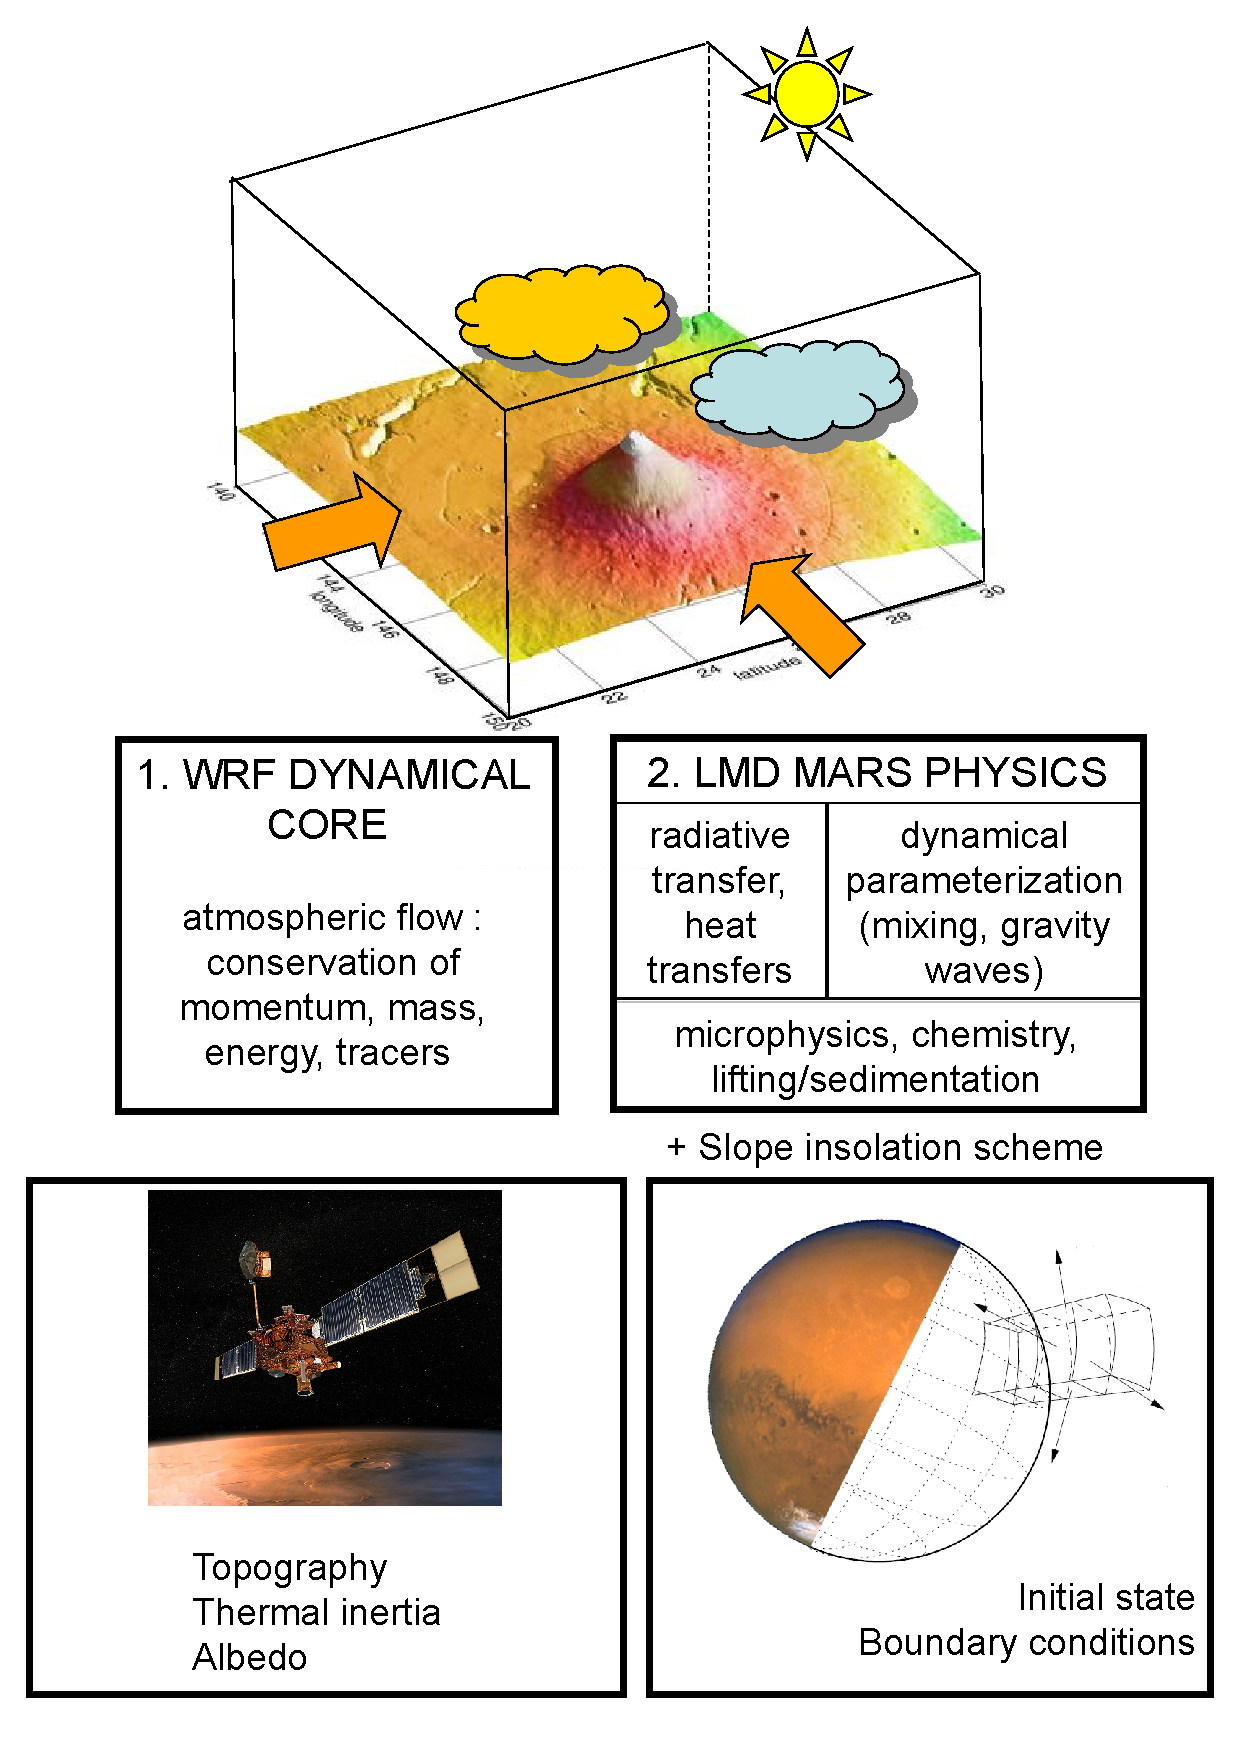
\includegraphics[width=0.99\textwidth]{meso.pdf} 
\caption{\label{modelstructure} An illustration of the LMD Martian Mesoscale Model design and capabilities.}
\end{figure}
\end{center}

\mk
\section{Dynamical core}

\sk
The numerical integration of the atmospheric fluid dynamic equations is performed in meteorological models by the dynamical core. The LMD Martian Mesoscale Model dynamical core is based on the stable and carefully tested, fully parallellized, Advanced Research Weather Research and Forecasting model (hereinafter referred as ARW-WRF) [\textit{Skamarock et al.}, 2005, 2008\nocite{Skam:08}\nocite{Skam:05}], developed for terrestrial applications at NCEP/NCAR (version 2.2.1 - November 2007).

\sk
The ARW-WRF mesoscale model integrates the fully compressible non-hydrostatic Navier-Stokes equations in a specific area of interest on the planet. Since the mesoscale models can be employed to resolve meteorological motions less than few kilometers, a scale at which the vertical wind acceleration might become comparable to the acceleration of gravity, hydrostatic balance cannot be assumed, as is usually done in General Circulation Models (GCMs).

\sk
Mass, momentum, entropy, and tracer conservation are ensured by an explicitly conservative flux-form formulation of the fundamental equations, based on mass-coupled meteorological variables (winds, potential temperature, tracers). Alternatively, these variables are recast into a reference profile plus a perturbation to reduce truncation errors [\textit{Skamarock et al.}, 2008]\nocite{Skam:08}. Tracer transport can be computed by an additional forward-in-time scheme based on the Piecewise Parabolic Method [\textit{Carpenter et al.}, 1990]\nocite{Carp:90}, with positive definite and monotonic properties
[\textit{Skamarock et al.}, 2006]\nocite{Skam:06}.

\sk
In the vertical dimension, the equations are projected, as suggested by \textit{Laprise} [1992]\nocite{Lapr:92}, on terrain-following mass-based coordinates (``eta levels"): $\eta = (\pi-\pi_t) / (\pi_s-\pi_t)$ where $\pi$ is the hydrostatic component of the pressure, $\pi_s$ the value at the surface and $\pi_t$ the (constant) upper boundary value. As shown in \textit{Laprise} [1992]\nocite{Lapr:92} and \textit{Janjic et al.} [2001]\nocite{Janj:01}, the choice of such vertical coordinates enables the integration of the ARW-WRF equations either in full non-hydrostatic mode or under the hydrostatic assumption. At the top of the domain, a free relaxation condition to zero vertical velocity is imposed (gravity wave absorbing layers can be defined as well).

\sk
In the horizontal dimension, the dynamical solver is available with three possible projections on the planetary sphere: Mercator (suitable for equatorial regions),  Lambert Conformal (for mid-latitudes),  and Polar Stereographic (for high-latitudes). Projections are defined by map scale factors, ensuring a regular computational grid whatever the map projection should be. Polar simulations are therefore devoid of any pole singularity, an usual drawback of the GCMs that requires the use of additional filtering. The spatial discretization is an Arakawa C-grid, where normal velocities are staggered one-half grid length from the thermodynamic variables [\textit{Arakawa}, 1966]\nocite{Arak:66}.

\sk
In the temporal dimension, a third-order Runge-Kutta integration scheme is employed for improved numerical accuracy and stability: the maximum stable Courant Friedrichs Lewy (CFL) numbers for advection are increased by a factor of two compared to the regular leapfrog integration scheme [\textit{Skamarock et al.}, 2008]. A time-splitting integration technique is implemented to prevent the meteorologically insignificant acoustic motions from triggering numerical instabilities [\textit{Klemp et al.}, 2007]\nocite{Klem:07}. Additional filters for acoustic external and internal modes damp residual instabilities possibly arising in the acoustic step integration.

\sk
In the ARW-WRF Runge-Kutta time-integration scheme, while pressure gradient and divergence terms are simply second order and centered, spatial discretizations of the advection terms for momentum, scalars and geopotential are 2nd through 6th order accurate [\textit{Wicker and Skamarock}, 2002]\nocite{Wick:02}. Martian simulations are performed with a 5th order discretized advection. One peculiarity of the odd-order advection discretization is the inherent inclusion of a dissipation term [\textit{Hundsdorfer et al.}, 1995]\nocite{Hund:95} with a coefficient proportional to the Courant number.

\sk
However, as was pointed out by \textit{Knievel et al.} [2007]\nocite{Knie:07}, this odd-ordered implicit scheme is not diffusive enough in low-wind or neutral/unstable stratification, and numerical noise in the wind fields might reach amplitudes comparable to the simulated winds. Such noise was found to be significant in the Martian case under near-surface afternoon superadiabatic conditions. The standard Martian simulations thus include the additional 6th order diffusion scheme developed by \textit{Knievel et al.}, with a removal parameter set for Martian applications to $20\%$ of the $2\,\Delta x$ noise in one timestep. While reducing the numerical noise near the surface to almost undiscernable amplitudes, the additional Knievel diffusion has little effect on the simulated meteorological fields.

\sk
Particular adaptations were required to use the ARW-WRF dynamical solver in the Martian environment. Physical constants, such as the acceleration of gravity and the planetary rotation rate, were converted to the Martian values. Vegetation and ocean-related variables were not used, and replaced with variables more suitable for the Martian applications (e.g., thermal inertia). Martian dates are given by the aerocentric solar longitude $L_s$, which indicates the position of Mars with respect to the Sun (0, 90, 180, 270 degrees are, respectively, the beginning of the northern hemisphere spring, summer, fall and winter). The terrestrial calendar was thus replaced with the LMD-GCM Martian calendar built on 669 Martian sols split in 12 ``aerocentric longitude"-based months (each of them is $L_s=30^{\circ}$ long, and thus encloses an irregular number of Martian sols due to the high eccentricity of the orbit), and one hour was defined as $1/24$ sol.

\mk
\section{Martian physics}

\sk
In any meteorological model, the 3D dynamical core is coupled with parameterization schemes (most often 1D) to compute at each grid point of the simulation domain the particular physics of the considered planetary environment: diabatic forcing of the atmospheric circulation (radiative transfer, soil thermal diffusion); sub-grid scale dynamical parameterizations (Planetary Boundary Layer [PBL] diffusion and mixing, convective adjustment); tracer sources and sinks (microphysical processes, chemistry, dust sedimentation and lifting). The LMD-MGCM complete physical parameterizations are interfaced with the adapted ARW-WRF dynamical core, described in the previous section, by a new ``driver" that is built on the same principles as the ARW-WRF terrestrial parameterization schemes, which are all switched off for the Martian applications. Thus, the LMD Martian Mesoscale Model shares the same comprehensive physical parameterizations as the LMD-MGCM, in order to simulate the Martian dust, CO$_2$, H$_2$O and photochemistry cycles [\textit{Forget et al.}, 1999; \textit{Montmessin et al.}, 2004; \textit{Lefevre et al.}, 2004].

\sk
\subsection{Physical parameterizations}

\sk
The radiative transfer in the model accounts for CO$_2$ gas infrared absorption/emission [\textit{Hourdin et al.}, 1992]\nocite{Hour:92} and visible and infrared dust absorption, emission and diffusion [\textit{Forget et al.}, 1998, 1999]\nocite{Forg:98grl}. Description of the CO$_2$ condensation processes in the model can be found in \textit{Forget et al.} [1998b]\nocite{Forg:98}. Thermal conduction in the soil is simulated by the 11-layer soil model developed by \textit{Hourdin et al.} [1993]\nocite{Hour:93} for Mars (soil density and soil specific heat capacity are set as constants). Turbulent closure is based on turbulent viscosity with coefficients calculated from the ``$2.5$-order" scheme by \textit{Mellor and Yamada} [1982]\nocite{Mell:82}, improved by \textit{Galperin et al.} [1988]\nocite{Galp:88}. In the case where vertical mixing is handled in the independent 1D physical packages, the native vertical mixing schemes in the ARW-WRF dynamical core are switched off, and the most appropriate choice for explicit horizontal diffusion is the built-in ARW-WRF scheme based on horizontal deformation [\textit{Smagorinsky}, 1963]\nocite{Smag:63}.

\sk
Recent improvements on the radiative transfer computations [\textit{Dufresne et al.}, 2005]\nocite{Dufr:05}, on the slope irradiance estimations [\textit{Spiga and Forget}, 2008]\nocite{Spig:08grl}, on the dust lifting and sedimentation [\textit{Forget et al.}, 1999b\nocite{Forg:99icm5}; \textit{Newmann et al.}, 2002]\nocite{Newm:02a}, on the water cycle and water ice clouds [\textit{Montmessin et al.}, 2004]\nocite{Mont:04}, and on the photochemical species [\textit{Lefevre et al.}, 2004]\nocite{Lefe:04}, particularly ozone [\textit{Lefevre et al.}, 2008]\nocite{Lefe:08}, are also natively included in the LMD Martian Mesoscale Model. The non-local thermodynamic equilibrium (NLTE) parameterizations for thermosphere applications [\textit{Gonz\'alez-Galindo et al.}, 2005\nocite{Gonz:05}] as well as estimations of the atmospheric exchanges with the Martian regolith [\textit{B\"ottger et al.}, 2005]\nocite{Bott:05}, are also available in the model.

%\sk
%Upcoming improvements of the LMD-MGCM physics [\textit{Forget et al.}, 2007]\nocite{Forg:07emsec}, following the recent measurements by instruments onboard Mars Express (MEx) and MRO, will be included in the LMD Martian Mesoscale Model too. Examples of future parameterizations that will be added in both models are the radiative effects of water ice clouds, which could significantly modify the atmospheric temperatures [\textit{Wilson et al.}, 2007]\nocite{Wils:07}, and the new dust radiative properties derived from recent measurements by the OMEGA instrument onboard MEx [\textit{M\"a\"att\"anen et al.}, 2008]\nocite{Maat:08} and the CRISM instrument onboard MRO [\textit{M.~J. Wolff and M. Vincendon}, personal communication, 2008].

\sk
Two physical parameterizations of the LMD-MGCM, specifically designed for synoptic-scale meteorological applications, are not used in the mesoscale applications.

\sk
Firstly, in the mesoscale domain, the topographical field is described with horizontal resolutions from tens of kilometers to hundreds of meters. The \textit{Lott and Miller} [1997]\nocite{Lott:97} subgrid-scale topographical drag parameterization and the \textit{Miller et al.} [1989]\nocite{Mill:89} gravity-wave drag scheme can thus be switched off, as the topographical influence on the atmospheric flow is computed by the dynamical core at the chosen mesoscale resolutions.

\sk
Secondly, in order to ensure numerical stability, and to account for subgrid-scale mixing processes insufficiently handled in the PBL scheme, it is usually necessary to modify any unstable layer with negative potential temperature gradients (an usual near-surface situation during Martian afternoons) into a neutral equivalent [\textit{Hourdin et al.}, 1993]. As pointed out by \textit{Rafkin} [2003b]\nocite{Rafk:03adj}, the use of such an artificial convective adjustment scheme might be questionable in Martian atmospheric models, should they be GCMs or mesoscale models. Since numerical stability is ensured in the LMD Martian Mesoscale Model by choosing the appropriate dynamical timestep with respect to the CFL condition, and using the aforementioned ARW-WRF nominal filters and diffusion schemes, the convective adjustment scheme used in the LMD-MGCM can thus be switched off in the LMD Martian Mesoscale Model. 

\mk
\subsection{Physical timestep}

\sk
Invoking physical packages often with respect to the dynamical computations was found to be necessary to accurately account for near-surface friction effects where the wind acceleration is particularly high, typically in regions of strong Martian topographically-driven circulation. In such areas, if the ratio between the physical timestep and the dynamical timestep is above $\sim 5$, the model predicts winds spuriously increasing with the chosen ratio and varying with the horizontal resolution. On the contrary, if this ratio is less than $\sim 5$, the simulated winds neither vary significantly with the chosen ratio nor with the horizontal resolution.

\sk
A ratio equal to 1 is chosen in the standard LMD Martian Mesoscale Model simulations. This choice is in conformity with the strategy adopted in the terrestrial ARW-WRF model. Besides, computing the physical parameterizations at the same frequency as the dynamical integration is profitable to some physical parameterizations, such as the formation of clouds (which is sensitive to rapid temperature change). Note that radiative transfer computations are usually carried out less often to save computational time.

\sk
When the ratio between the physical timestep and the dynamical timestep is superior to 1, two distinct strategies could be adopted. Interestingly, we found that splitting the physical tendency in equal parts and blending it with the dynamical tendency at each dynamical timestep computation is slightly more stable (understand: allows for higher dynamical timesteps) than applying the whole physical tendency when the physical parameterizations are computed, and letting the dynamical core naturally evolve until the next physics call. However, an analysis of the simulated meteorological fields in both cases does not reveal significant differences.

\mk
\section{Initial and boundary conditions}
\label{ssc:inibdy}

\mk
\subsection{Starting state and horizontal boundaries}

\sk
Mesoscale simulations can be performed in a limited domain anywhere on the planet. Thus, boundary conditions for the main meteorological fields (horizontal winds, temperature, tracers) have to be provided during the simulations, in addition to an atmospheric starting state. Idealized simulations usually require the use of periodic, symmetric or open boundary conditions, whereas real-case simulations need specified climatologies at the boundaries.

\sk
The specified boundary conditions and the atmospheric starting state are derived from previously performed $64\times48\times25$ (i.e., horizontal resolution of $5.625^{\circ}$ in longitude and $3.75^{\circ}$ in latitude, model top $\sim$~80~km~altitude) LMD-MGCM simulations which have reached equilibrium, typically after $\sim 10$ simulated years. GCM results are often used every Martian hour to constrain the mesoscale model at the domain boundaries. Temporal interpolations to each mesoscale timestep and spatial interpolations on the mesoscale domain are performed from the LMD-MGCM inputs. A relaxation zone of a given width (user-defined, usually 5 grid points) is implemented at the boundaries of the ARW-WRF domain to enable both the influence of the large-scale fields on the limited area, and the development of the specific mesoscale circulation inside the domain. The interpolations and the use of a relaxation zone prevent the prescribed meteorological fields at the lateral boundaries from having sharp gradients and from triggering spurious waves or numerical instabilities (the situation where the relaxation zone crosses steep topographical gradients should however be avoided).

\mk
\subsection{Nesting or single-domain strategy ?}
\label{ssc:nestingvalid}

\sk
The model includes one-way and two-way (or ``feedback") nesting capabilities. The nested simulations feature two kinds of domains where the meteorological fields are computed: the "parent" domain, with a large geographical extent, a coarse grid resolution, and specified boundary conditions, and the "nested" domains, centered in a particular zone of interest, with a finer grid resolution, and boundary conditions provided by its parent domain.

\sk
The nesting capabilities can be used only if deemed necessary, and single-domain simulations may be the primary type of run performed.

\sk
Firstly, employing the same physical parameterizations in the mesoscale model computations and in the GCM simulations defining the boundary and initial conditions, ensures a very consistent meteorological forcing at the boundaries of the mesoscale domain. This assumption was not denied by further examination of the performed simulations: mesoscale predictions are not unrealistically departing from the LMD-MGCM prescribed fields at the boundaries, and the mesoscale influence naturally adds to the synoptic (large-scale) tendency communicated at the boundaries. 

\sk
Secondly, the single-domain approach is appropriate as long as the variations of near-surface winds, pressure and temperature induced by ``passing" thermal tides through the east-west boundaries are not unrealistic. This criterion is specific to Martian mesoscale modeling and was described by \textit{Tyler et al.} [2002]. In the various simulations performed with the LMD Martian Mesoscale Model, a likely spurious influence of the passing thermal tides was only detected in the near-surface meteorological fields calculated at the $\sim 5$ near-boundaries grid points. The amplitudes of the departures were negligible ($\delta T \apprle 3$~K; $\delta u, \delta v \apprle 5\%$) and did not require the use of domains nested inside one semi-hemispheric parent domain [\textit{Tyler et al.}, 2002]. However, the analysis of the simulated fields at the near-boundaries grid points should be carried out with caution when choosing the single-domain approach. A practical solution to this drawback is to define a large domain, centered on the chosen area of interest, with a sufficient number of grid points ($75 \times 75$ being a minimal requirement).

\sk
Thirdly, \textit{Dimitrijevic and Laprise} [2005]\nocite{Dimi:05} showed, by the so-called ``Big Brother" approach, that the single-domain approach yields unbiased results when the boundary forcing involves a minimum of $\sim 8-10$ GCM grid points. Thus, given the resolution of the GCM fields used to constrain the LMD Martian Mesoscale Model, single-domain simulations with, for instance, a horizontal resolution of $20$~km shall be performed on at least $133 \times 88$ grid points. \textit{Antic et al.} [2006]\nocite{Anti:06} found that the ``$8-10$ grid points" limit can be lowered in situations of complex topography, because the dynamical influence of these mesoscale features is responsible for the larger part of the mesoscale circulation in the domain. Such situations are rather common on Mars, and the aforementioned ``minimal" grid can be of slightly smaller horizontal extent in areas such as Olympus Mons or Valles Marineris.

\sk
Thus the sizes of the simulation grids have to be chosen in order to ensure the applicability of the single-domain approach. The nesting technique is used only when defining a single domain with sufficient geographical extent would have required too many grid points to handle the computations within reasonable CPU time. For instance, with ``$64 \times 48$" GCM simulations as boundary conditions, the use of the single-domain strategy to model the Arsia Mons circulation at $5$ km resolution imposes a simulation grid of at least $531 \times 354$ points. The nesting technique is more suitable for this kind of simulation.

\mk
\subsection{Surface fields}

\sk
Surface static data intended for the mesoscale domain are extracted from maps derived from recent spacecraft measurements: 64 pixel-per-degree (ppd) MOLA topography [\textit{Smith et al.}, 2001]\nocite{Smit:01mola}, 8 ppd MGS/Thermal Emission Spectrometer (TES) albedo [\textit{Christensen et al.}, 2001]\nocite{Chri:01}, 20 ppd TES thermal inertia [\textit{Putzig and Mellon}, 2007]\nocite{Putz:07}. A smoother composite thermal inertia map derived from \textit{Palluconi and Kieffer} [1981]\nocite{Pall:81}, \textit{Mellon et al.} [2000]\nocite{Mell:00} and \textit{Vasavada et al.} [2000]\nocite{Vasa:00} can be alternatively used for better continuity with LMD-MGCM simulations. Except for CO$_2$ ice covered areas, emissivity is set to $0.95$. The roughness length $z_0$ is set to the constant value of $1$~cm, but further versions of the model will use spatially-varying $z_0$ [\textit{H\'ebrard et al.}, 2007]\nocite{Hebr:07}. Initial values for time-varying surface data, such as CO$_2$ and H$_2$O ice on the surface and soil temperatures, are derived from the GCM simulations. The latter initialization reduces the spin-up time for surface temperature to roughly one simulated sol.

\sk
The LMD Martian Mesoscale Model has the complete ability to simulate the dust cycle (lifting, sedimentation, transport). However, the high sensitivity of the results to the assumptions made on threshold wind stress and injection rate [\textit{Basu et al.}, 2004]\nocite{Basu:04} leads us to postpone these issues to future studies. Instead, similarly to the reference LMD-MGCM simulations, dust opacities are prescribed in the mesoscale model from 1999-2001 TES measurements, thought to be representative of Martian atmospheric conditions outside of planet-encircling dust storm events [\textit{Montabone et al.}, 2006]\nocite{Mont:06luca}. In the vertical dimension, as described in \textit{Forget et al.} [1999], and in accordance with the general consensus of well-mixed dust in equilibrium with sedimentation and mixing processes [\textit{Conrath}, 1975]\nocite{Conr:75}, dust mixing ratio is kept constant from the surface up to a given elevation $z_{\textrm{\tiny{max}}}$ above which it rapidly declines. Both in the nominal GCM and mesoscale simulations, $z_{\textrm{\tiny{max}}}$ as a function of areocentric longitude and latitude is calculated from the ``MGS scenario" [\textit{Forget et al.}, 2003]\nocite{Forg:03}.

\mk
\subsection{Vertical interpolation}

\sk
In the process of initialization and definition of boundary conditions, the vertical interpolation of GCM meteorological fields to the terrain-following mesoscale levels must be treated with caution. While deriving the near-surface meteorological fields from GCM inputs, one may address the problem of underlying topographical structures at fine mesoscale horizontal resolution, e.g., a deep crater that is not resolved in the coarse GCM case.

\sk
A crude extrapolation of the near-surface GCM fields to the mesoscale levels is usually acceptable for terrestrial applications. On Mars, owing to the low density and heat capacity of the Martian atmosphere, the surface temperature is to first order controlled by radiative equilibrium, and thus it is left relatively unaffected by variations of topography [e.g. \textit{Nayvelt et al.}, 1997]\nocite{Nayv:97}. A practical consequence, which renders an extrapolation strategy particularly wrong on Mars, is that the near-surface temperature and wind fields vary much more with the distance from the surface than with the absolute altitude above the areoid (or equivalently with the pressure level). Initial tests carried out with the extrapolation strategy showed that differences between temperatures at the boundaries and temperatures computed within the mesoscale domain close to these boundaries often reach $20-30$~K near the surface. An interpolation based only on terrain-following principles solves this problem near the surface but was found to lead to numerical instabilities at higher altitudes during the mesoscale integrations.

\sk
Therefore, input meteorological data need to be recast on intermediate pressure levels $P'$ with a low level smooth transition from terrain-following levels (for the near-surface environment) to constant pressure levels (for the free atmosphere at higher altitude). We thus have $P'(x,y)=\alpha + \beta \, P_s(x,y)$, $P_s$ being the surface pressure at the resolution of the GCM simulations. To ensure a realistic low-level transition, the technique described in \textit{Millour et al.} [2008]\nocite{Mill:08ddd}, based on high-resolution GCM results, is employed to calculate the $P'$ levels. The mesoscale surface pressure field $p_s$ is an input parameter of the method, since the near-surface adiabatic cooling over mountains and warming within craters are taken into account. Note that $p_s(x,y)$ is calculated from $P_s(x,y)$ on the basis of the high-resolution topography of the mesoscale domain $z(x,y)$ by $$p_s(x,y) = P_s(x,y) \, e^{ \frac{g \, [Z(x,y)-z(x,y)]}{R \, T(x,y)} }$$ \noindent where $Z(x,y)$ is the topography at the resolution of the GCM simulations, $R$ the gas law constant, $g$ the acceleration of gravity, and $T(x,y)$ the temperature predicted by the GCM $1$~km above the surface (see \textit{Spiga et al.} [2007]\nocite{Spig:07omeg}). Without reinterpolating the data, the intermediate pressure $P'$ levels are then simply converted into their mesoscale counterparts $p'$ by substituting $p_s$ for $P_s$ in the formula $P'(x,y)=\alpha + \beta \, P_s(x,y)$. Finally, the built-in ARW-WRF vertical interpolation onto the final mesoscale terrain-following levels can be performed, as the problem of extrapolation is solved by the use of the intermediate pressure levels $p'$.

\sk
The initial atmospheric state obtained through this ``hybrid" method ensures low-amplitude adjustments of the meteorological fields by the mesoscale model at the beginning of the performed simulations (i.e., in the first thousands of seconds). Furthermore, the continuity between the large-scale forcing and the mesoscale computations near the limits of the domain, as well as the numerical stability of the simulations, appear as significantly improved compared to methods either based on extrapolation (especially in areas of uneven terrains) or terrain-following interpolation.

%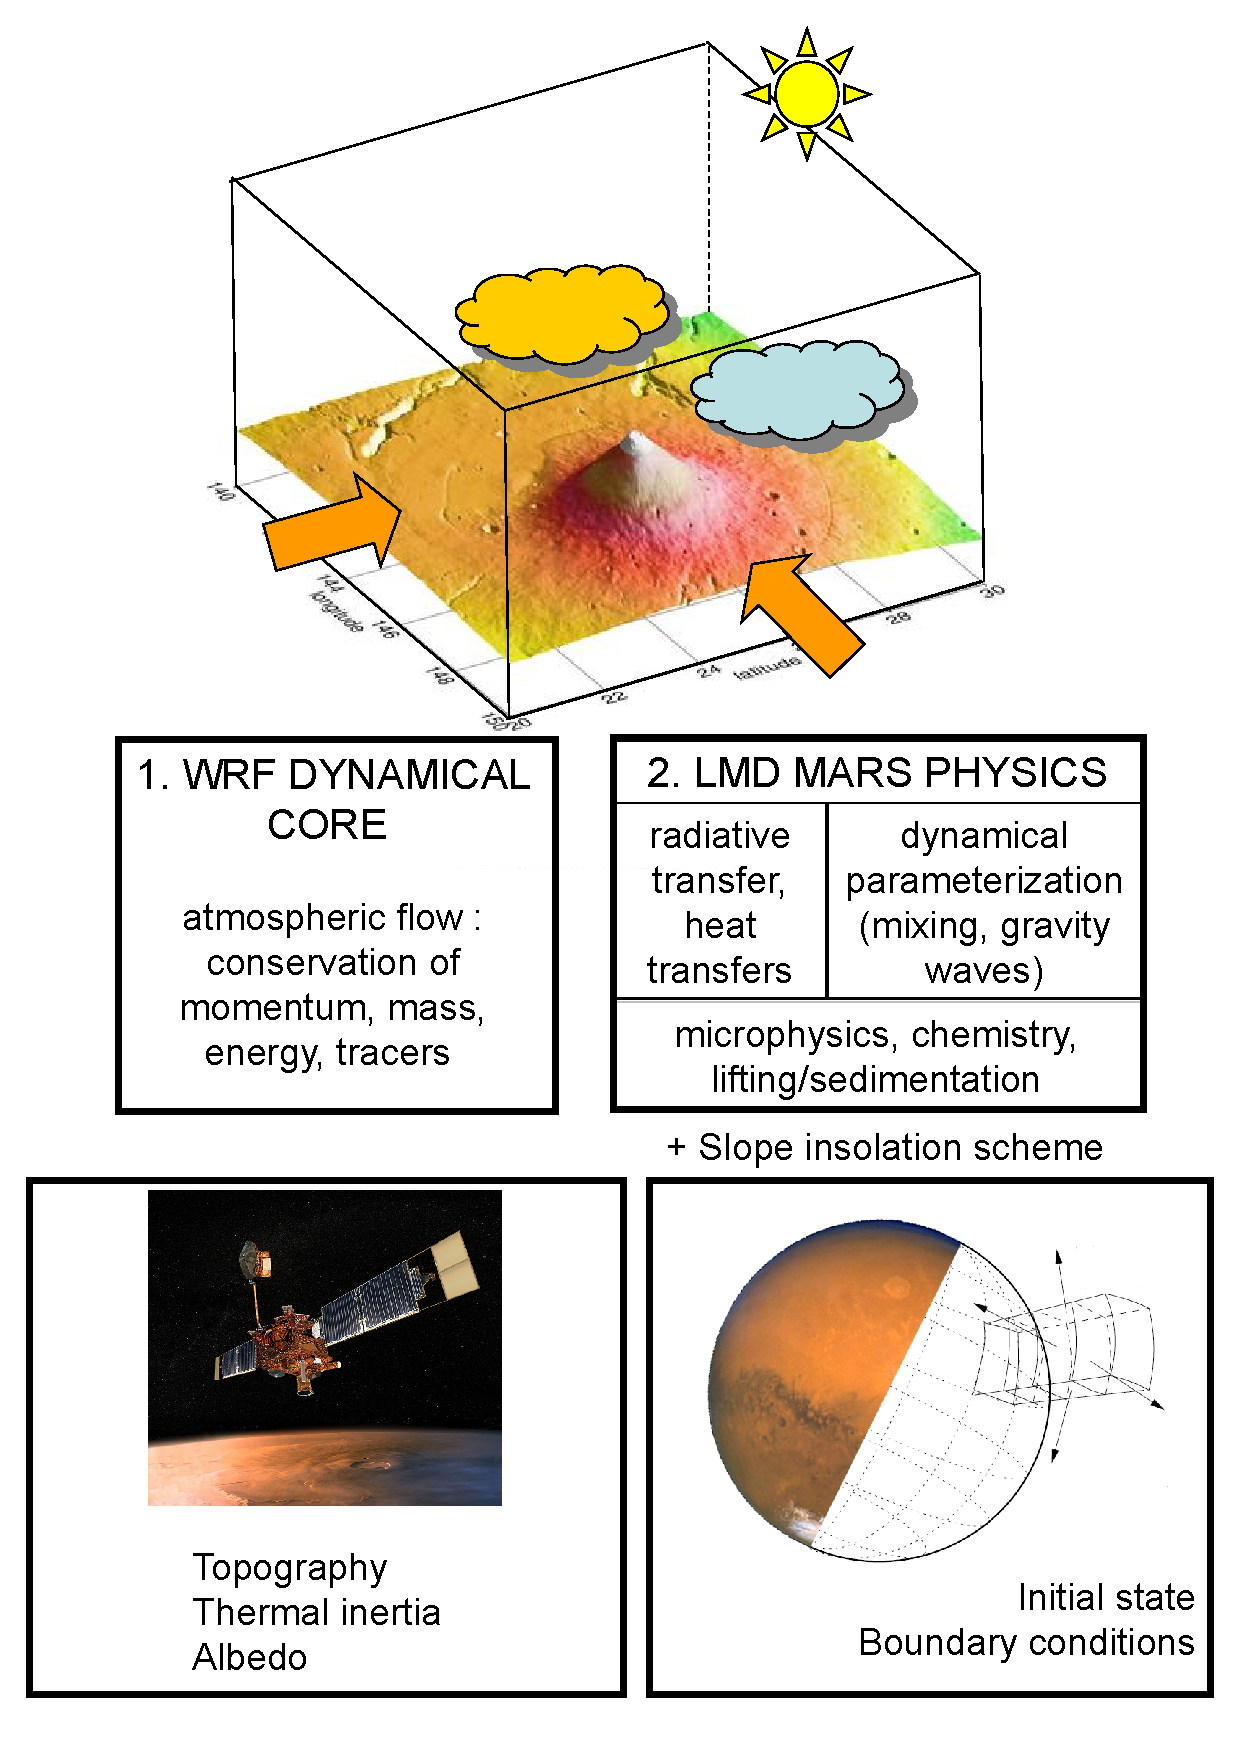
\includepdf[pages=1,offset=25mm -20mm]{meso.pdf}
\clearemptydoublepage

